\documentclass{article}
\usepackage{graphicx} % Required for inserting images

\title{Cooling Tower Project}
\author{Emma Li and Z Ling}
\usepackage{amsma   th,amssymb,amsthm,amsxtra,bbm,cancel,xcolor,enumitem,fancybox,graphicx,mathtools,multirow,titling,url,wasysym,mathcomp,tcolorbox,mathrsfs,tikz,}

\begin{document}

\maketitle

\section{AP Calculus BC\@ Determining the Amount of Concrete Needed for a Cooling Tower}

A common design for cooling towers is modeled by a branch of a hyperbola rotated about an axis. The design is used because of its strength and efficiency. Not only is the shape stronger than either a cone or cylinder, it takes less material to build. This shape also maximizes the natural upward draft of hot air without the need for fans.
How much concrete is needed to build a cooling tower that has a base $460$ft wide that is $442$ ft below the vertex if the top of the tower is $310$ ft wide and $123$ ft above the vertex? Assume the walls are a constant $5$in $= 0.42$ ft thick. See the figure below:
    \begin{center}
    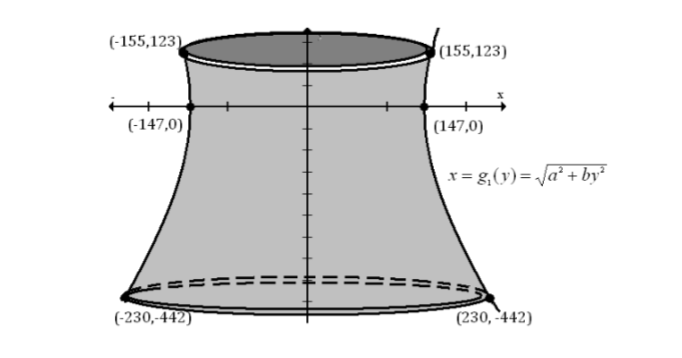
\includegraphics[scale=0.90]{Figure1.png}
    \end{center}

Answer the following questions. Explain your reasoning completely in complete sentences, using correct mathematical terminology.
\begin{enumerate}
    \item Show that the equation of the right branch of the hyperbola in the figure above is given
by $x=g_2(y) = \sqrt{a^2+by^2}$ where $a = 147$ and $b = 0.16$
\begin{proof}

The standard form of the equation for a hyperbola is $\frac{x^2}{a^2}-\frac{y^2}{b^2}=1$, where $a$ is half the length of the transverse axis ($x$-axis), and $b$ is half the length of the conjugate axis ($y$-axis). 

Since $a, b$ are used in the problem, for convenience's sake, replace $a,b$ with $c, d$, respectively, in the standard from the equation for a hyperbola. Manipulating this equation, we find:
\begin{align*}
    \frac{x^2}{c^2}-\frac{y^2}{d^2}&=1\\
    x^2-\frac{c^2y^2}{d^2}&=c^2\\
    x^2&=\frac{c^2y^2}{d^2}+c^2\\
    x&=\pm\sqrt{\frac{c^2y^2}{d^2}+c^2}
\end{align*}
Since we only want the right branch, we only take positive values of $x$, so we have
$$x=\sqrt{c^2+\frac{c^2}{d^2}y^2}$$

Since we know that the vertices of the hyperbola are $(-147, 0)$ and $(147,0)$, the length of the transverse axis is $294$. Thus $c=147$. 

Since $c^2$ is the only constant under the square root, $c^2$ is the same thing as $a^2$ in $g_2(y)$. Thus $a=c=147$.

Now we know that $x=g_2(y)=\sqrt{147^2+by^2}$, and we also know a few points on the right branch of the hyperbola. Thus, we can plug in these points to solve for $b$
\begin{align*}
    155&=\sqrt{147^2+b(123)^2}\\
    155^2&=147^2+b(123)^2\\
    155^2-147^2&=b(123)^2\\
    \frac{155^2-147^2}{123^2}&=b\\
    b&=\frac{155^2-147^2}{123^2}\\
    b&\approx0.16
\end{align*}

Thus it has been shown that $a=147$ and $b\approx0.16.$

\end{proof}


\item Find the volume of the solid of revolution obtained by revolving the area enclosed by $x=g_2(y)$ from $y = -442$ to $y = 123$ about the y-axis.

\begin{proof}

We can simply integrate with respect to y sing the disk method with the radius being $g_2(y)$ and  $A(x) = \pi(g_2(y))^2$, so integrating from the given bounds gives

$$\int_{-442}^{123} \pi(\sqrt{147^2+.16y^2})^2 \,dy = \pi\int_{-442}^{123} (147^2+.16y^2) \,dy \approx 53,135,993.155$$ 

Thus, the volume is approximately $\boxed{53,135,993.155\text{ ft}^3}$. 

\end{proof}

\item Using the fact that the walls are 0.42 ft thick, show that the equation of the interior
hyperbola is given by $x=g_1(y)=\sqrt{q^2+ry^2}$ where $q = 146.58$ and $r = 0.16$. See figure
below
   \begin{center}
    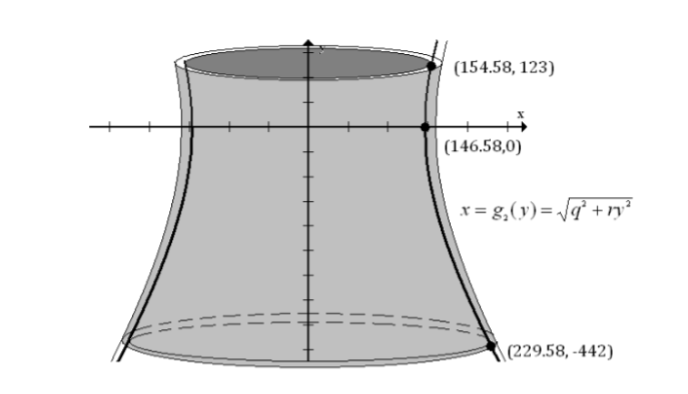
\includegraphics[scale=0.90]{Figure2.png}
    \end{center}
\begin{proof}
The standard form of the equation for a hyperbola is $\frac{x^2}{a^2}-\frac{y^2}{b^2}=1$, where $a$ is half the length of the transverse axis ($x$-axis), and $b$ is half the length of the conjugate axis ($y$-axis). 

Since $a, b$ are used for $g_2(y)$, replace these variables with $c, d$. Manipulating this equation, we find:
\begin{align*}
    \frac{x^2}{c^2}-\frac{y^2}{d^2}&=1\\
    x^2-\frac{c^2y^2}{d^2}&=c^2\\
    x^2&=\frac{c^2y^2}{d^2}+c^2\\
    x&=\pm\sqrt{\frac{c^2y^2}{d^2}+c^2}\\
    x&=\sqrt{c^2+\frac{c^2}{d^2}y^2}\\
\end{align*}

Since we know that the walls are $0.42$ ft thick, the length of the transverse axis of the inner hyperbola is $294-0.42\cdot2=293.16$. Thus $c=146.58$. 

Since $c^2$ is the only constant under the square root, $c^2$ is the same thing as $q^1$ in the $g_1(y)$. Thus $q=c=146.58$.

Now we know that $x=g_1(y)=\sqrt{146.58^2+ry^2}$, and we also know a few points on the right branch of the hyperbola. Thus, we can plug in these points to solve for $r$
\begin{align*}
    154.58&=\sqrt{146.58^2+r(123)^2}\\
    154.58^2&=146.58^2+r(123)^2\\
    154.58^2-146.58^2&=r(123)^2\\
    \frac{154.58^2-146.58^2}{123^2}&=r\\
    r&=\frac{154.58^2-146.58^2}{123^2}\\
    r&\approx0.16
\end{align*}

Thus it has been shown that $q=146.58$ and $r\approx0.16.$



\end{proof}
\item Find the volume of the solid of revolution obtained by revolving the area enclosed by $x =
g_1(y)$ from $y = -442$ and $y = 123$ about the $y$-axis.

\begin{proof}

Using the same method as in number 2, we can use the disk method with respect to y with the radius as $g_1(y)$ and $A(x) = \pi g_1(y)^2$, so by integrating from the given bounds,

$$ \int_{-442}^{123} \pi(\sqrt{146.58^2+.16y^2})^2 \,dy = \pi \int_{-442}^{123} (146.58^2+.16y^2) \,dy $$ $$\approx 52,917,129.283$$

Thus, the volume is approximately $\boxed{52,917,129.283\text{ ft}^3}$. 
\end{proof}

\item Now determine the volume (in cubic feet) of concrete required for the cooling tower.

\begin{proof}
The volume of the outer graph revolved around the y-axis minus the volume of the inner graph revolved around the y-axis must be the area in between, which is the volume of the wall. So by simple arithmetic
    $$53,135,993.155 - 52,917,129.283 = 218,863.872$$ 
so the volume of concrete required for the cooling tower is approximately $\boxed{218,863.872\text{ ft}^3}$.
\end{proof}


\item Do an Internet search to find the cost of concrete. How much will the concrete used in the cooling tower cost?

\begin{proof}
    Assuming the cooling tower is constructed with the cheapest concrete from Home Depot, each cubic foot of concrete costs around $10$ dollars. Thus the total cost of the cooling tower should be
    $$218,863.872\text{ ft}^3\cdot\frac{10\text{ dollars}}{\text{ft}^3}=\boxed{2,188,638\text{ dollars}}$$  
\end{proof}

\item Write a report for an audience that is not familiar with cooling towers summarizing the
findings in $\#1-6$.

print('Hello World')

\end{enumerate}



\end{document}
